
\documentclass{acm_proc_article-me}

\usepackage[none]{hyphenat}
\sloppy

\begin{document}
\conferenceinfo{\textit{MediaEval 2014 Workshop,}}{October 16-17, 2014, Barcelona, Spain}

\title{DCLab at MediaEval2014 Retrieving Diverse \\ Social Images Task}

\numberofauthors{3}

\author{
\alignauthor
Zsombor Par\'oczi\\
       \affaddr{Inter-University Centre for Telecommunications and Informatics}\\
       \email{paroczi@tmit.bme.hu}
\alignauthor
B\'alint Fodor\\
       \affaddr{Inter-University Centre for Telecommunications and Informatics}\\
       \email{balint.fodor@aut.bme.hu}
\alignauthor
G\'abor Sz\H ucs \\
       \affaddr{Inter-University Centre for Telecommunications and Informatics}\\
       \email{szucs@tmit.bme.hu}
}

\maketitle
\begin{abstract}
TODO abstract
\end{abstract}

\section{Introduction}

Many potential tourists do websearches when they try to find more information about a place he (or she) is potentially visiting. These people have only a vague idea about the location, knowing the name of the place. Our aim is to help them by providing a set of photos, as summary of the different views of the location. 
In the official challenge (Retrieving Diverse Social Images at MediaEval 2014: Challenge, Dataset and Evaluation) \cite{ionescu2014retrieving} a ranked list of location photos retrieved from Flickr (using text information) is given, and the task is, to refine the results by providing a set of images that are both relevant and provide a diversified summary. The diversity means that images can illustrate different views of the location at different times of the day/year and under different weather conditions, creative views, etc. The refinement and diversification process can be based on the social metadata associated with the collected photos in the data set~\cite{ionescu2014div400} and/or on the visual characteristics of the images. The initial results are typically noisy and redundant because of social media platform~\cite{radu2014hybrid}, where the large variety comes from very different users. 

The goodness of the refinement process can be measured using the precision and diversity metric~\cite{Taneva:2010:GRP:1718487.1718541}. Earlier we have solved a very similar problem by diversification of initial results using clustering~\cite{szHucs2013bmemtm}, but our solution was focused on diversification only. The largest development of this paper is that we focus on both the relevance and diversity.

\section{Reordering System}

We took five approaches to generate the final reordering of the inital search result. This required five different systems that share similar components. All the systems take the inital ordering as the input along with the visual feature descriptors and the textual descriptors corresponding to the images. In each case the relevancy of all images are estimated, the images are grouped into clusters and based on this two type of information the final ordering is determined.

\begin{table}[h]
\begin{tabular}{|c|c|c|}
	\hline 
	run name & relevance & clustering\tabularnewline
	\hline 
	\hline 
	run1 & devset avg & visual descriptors\tabularnewline
	\hline 
	run2 & devset avg & textual descriptors\tabularnewline
	\hline 
	run3 & devset avg & visual+textual descriptors\tabularnewline
	\hline 
	run4 & devset avg scaled with user credibility & visual+textual descriptors\tabularnewline
	\hline 
	run5 & combined devset avg and credibility information & visual+textual descriptors\tabularnewline
	\hline 
\end{tabular}
\caption{TODO caption}
\end{table}

\subsection{Relevance Scoring}

For every $k$th place in the orderings of the developer data set we calculated the probability of the item at the $k$th place is beeing relevant. Before giving the formal definition let denote the set of all orderings in the developer set as $L$, the $k$th element of the ordering $l \in L$ as $l_k$ and the binary function of the relevancy (based on the ground truth data) as $r_{gt}(l_k)$. Then $p_k$, the estimated probability of the $k$th element in an ordering is relevant:
$p_k = \frac{1}{|L|}\sum_{l \in L}r_{gt}(l_k)$.

When processing an ordering (from the test data set) we give the relevance score of $p_k$ to the $k$th element of the ordering.

\subsection{Clustering}

TODO text clustering

The provided data sets contains visual feature descriptors (color moments, histogram of oriented gradients, etc.) in csv files. First, we merged the descriptors into a long feature vector, one vector for each image. The clustering is done on a per ordering basis, so the feature vector is calculated for every image in an ordering. Then the components of the vectors are normalized to bring all the data to the same scale. The vectors are clustered with the K-means algorithm by trying all clustering number parameters from 6 to 18. For every clustering the silhouette score~\cite{rousseeuw1987silhouettes} is calculated and the best instance is selected.

Clusterings based on textual and visual data can differ, but merging the two results can be beneficial. Having two clustering functions $c_1(x)$ and $c_2(x)$ that are mapping an image id to a cluster label, one can construct $c_3(x) = (c_1(x), c_2(x))$ that maps an image id to a new cluster labeled by the pair of the two original cluster labels. Note that the new label set is the Cartesian product of the two original cluster label sets.

\subsection{Final Ordering}

TODO

\section{Results and Conclusion}

\begin{table}[h]
\begin{tabular}{|l|r|r|r|}
	\hline 
	run name & P@20 & CR@20 & F1@20\tabularnewline
	\hline 
	\hline 
	VisClusterAvgRelevance & .7602 & .4107 & .5259\tabularnewline
	\hline 
	TextClusterAvgRelevance & .7809 & .4065 & .527\tabularnewline
	\hline 
	VisTextClusterAvgRelevance & .7756 & .4127 & .5305\tabularnewline
	\hline 
	VisTextClusterCredRelevance & .7415 & .3651 & .4819\tabularnewline
	\hline 
	VisTextClusterMixedRelevance & .7431 & .3682 & .4866\tabularnewline
	\hline 
\end{tabular}
\caption{Average results of the five approaches}
\end{table}

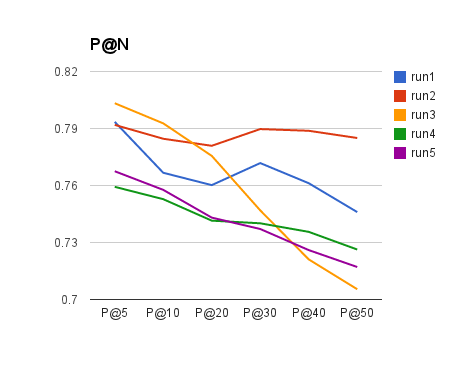
\includegraphics[width=0.9\linewidth]{p}


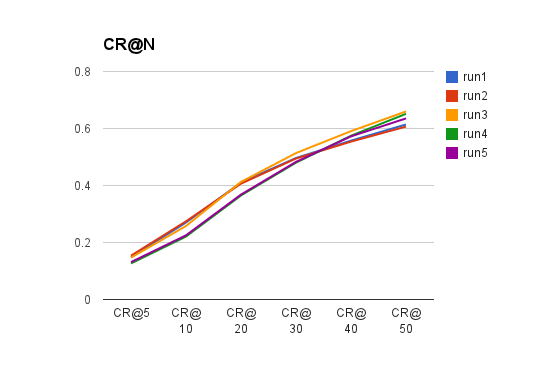
\includegraphics[width=0.9\linewidth]{cr}


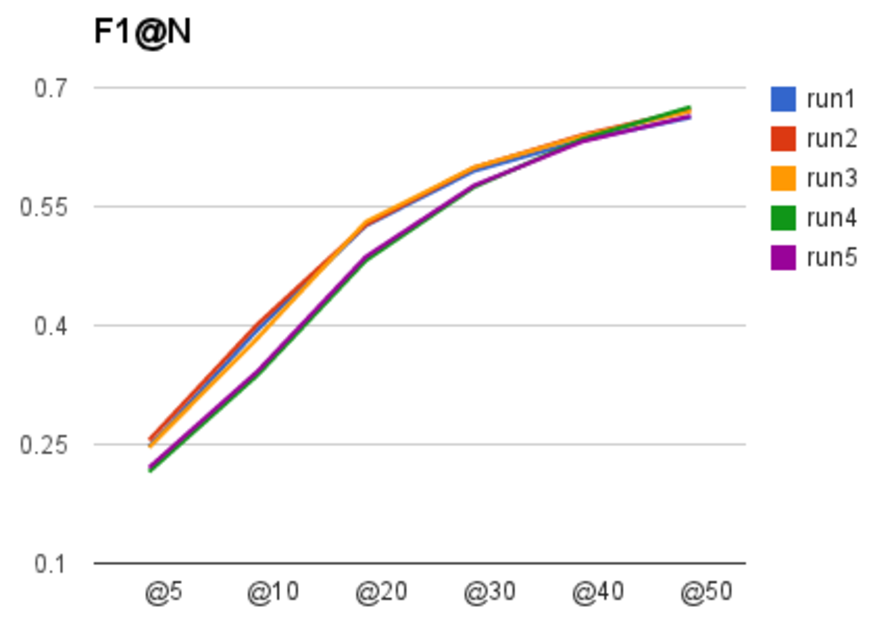
\includegraphics[width=0.9\linewidth]{f1}


% \subsection{Linking subtask}

% \begin{table}[h]
% \begin{tabular}{|c|c|c|c|}
% 	\hline 
% 	& P@5 & P@10 & P@20\tabularnewline
% 	\hline 
% 	\hline 
% 	Manual subtitles & .0750 & .0500 & .0312\tabularnewline
% 	\hline 
% 	LIMSI transcripts & .0444 & .0333 & .0167\tabularnewline
% 	\hline 
% 	LIUM transcripts & .0533 & .0400 & .0200\tabularnewline
% 	\hline 
% 	NST/Sheffield & .0400 & .0467 & .0233\tabularnewline
% 	\hline 
% 	All transc. and sub. & .0370 & .0407 & .0222\tabularnewline
% 	\hline 
% 	Manual subtitles (C2) & .1818 & .1000 & .0500\tabularnewline
% 	\hline 
% 	LIMSI transcripts (C2) & .0500 & .0625 & .0375\tabularnewline
% 	\hline 
% 	LIUM transcripts (C2) & .0526 & .0316 & .0184\tabularnewline
% 	\hline 
% 	NST/Sheffield (C2) & .0300 & .0350 & .0175\tabularnewline	
% 	\hline 
% 	All transc. and sub. (C2) & .0143 & .0250 & .0196\tabularnewline	
% 	\hline 
% \end{tabular}
% \caption{P@N result for the linking subtask}
% \end{table}

\section{Acknowledgments}

The publication was supported by the T\'AMOP-4.2.2.C-11/1/KONV-2012-0001 project. The project has been supported by the European Union, co-financed by the European Social Fund.

\bibliographystyle{abbrv}
\bibliography{sigproc}

\end{document}
